\begin{figure}[ht]
\begin{center}
\begin{adjustbox}{width=0.5\textwidth}



\tikzset{every picture/.style={line width=0.75pt}} %set default line width to 0.75pt        

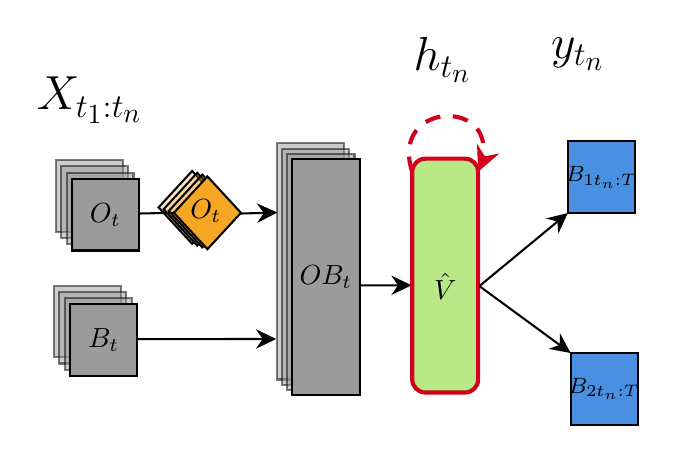
\begin{tikzpicture}[x=0.75pt,y=0.75pt,yscale=-1,xscale=1]
%uncomment if require: \path (0,300); %set diagram left start at 0, and has height of 300

%Shape: Diamond [id:dp06877884521197963] 
\draw  [fill={rgb, 255:red, 245; green, 166; blue, 35 }  ,fill opacity=0.25 ] (263.6,117.28) -- (279.77,134.81) -- (263.6,152.33) -- (247.43,134.81) -- cycle ;
%Shape: Diamond [id:dp5019197402707816] 
\draw  [fill={rgb, 255:red, 245; green, 166; blue, 35 }  ,fill opacity=0.25 ] (266.05,118.16) -- (282.22,135.68) -- (266.05,153.2) -- (249.89,135.68) -- cycle ;
%Shape: Diamond [id:dp6628494024847519] 
\draw  [fill={rgb, 255:red, 245; green, 166; blue, 35 }  ,fill opacity=0.25 ] (268.51,119.04) -- (284.68,136.56) -- (268.51,154.08) -- (252.34,136.56) -- cycle ;
%Shape: Rectangle [id:dp8304682723722553] 
\draw  [color={rgb, 255:red, 0; green, 0; blue, 0 }  ,draw opacity=0.5 ][fill={rgb, 255:red, 155; green, 155; blue, 155 }  ,fill opacity=0.5 ] (304.41,104.01) -- (336.92,104.01) -- (336.92,217.74) -- (304.41,217.74) -- cycle ;
%Shape: Rectangle [id:dp33657106031779216] 
\draw  [color={rgb, 255:red, 0; green, 0; blue, 0 }  ,draw opacity=0.5 ][fill={rgb, 255:red, 155; green, 155; blue, 155 }  ,fill opacity=0.5 ] (306.86,106.47) -- (339.38,106.47) -- (339.38,220.2) -- (306.86,220.2) -- cycle ;
%Shape: Rectangle [id:dp6698304713342962] 
\draw  [color={rgb, 255:red, 0; green, 0; blue, 0 }  ,draw opacity=0.5 ][fill={rgb, 255:red, 155; green, 155; blue, 155 }  ,fill opacity=0.5 ] (309.32,108.93) -- (341.84,108.93) -- (341.84,222.66) -- (309.32,222.66) -- cycle ;
%Shape: Diamond [id:dp7704333366065277] 
\draw  [fill={rgb, 255:red, 245; green, 166; blue, 35 }  ,fill opacity=1 ] (270.97,119.91) -- (287.13,137.43) -- (270.97,154.96) -- (254.8,137.43) -- cycle ;
%Straight Lines [id:da34159449213041837] 
\draw    (286.94,137.77) -- (301.65,137.38) ;
\draw [shift={(304.65,137.3)}, rotate = 178.49] [fill={rgb, 255:red, 0; green, 0; blue, 0 }  ][line width=0.08]  [draw opacity=0] (9.82,-4.72) -- (0,0) -- (9.82,4.72) -- (6.52,0) -- cycle    ;
%Straight Lines [id:da8208338090000002] 
\draw [fill={rgb, 255:red, 155; green, 155; blue, 155 }  ,fill opacity=1 ]   (215.09,198.3) -- (301.13,198.22) ;
\draw [shift={(304.13,198.22)}, rotate = 179.95] [fill={rgb, 255:red, 0; green, 0; blue, 0 }  ][line width=0.08]  [draw opacity=0] (9.82,-4.72) -- (0,0) -- (9.82,4.72) -- (6.52,0) -- cycle    ;
%Straight Lines [id:da7791621502079311] 
\draw [fill={rgb, 255:red, 155; green, 155; blue, 155 }  ,fill opacity=1 ]   (336.42,172.36) -- (366.33,172.35) ;
\draw [shift={(369.33,172.35)}, rotate = 179.97] [fill={rgb, 255:red, 0; green, 0; blue, 0 }  ][line width=0.08]  [draw opacity=0] (9.82,-4.72) -- (0,0) -- (9.82,4.72) -- (6.52,0) -- cycle    ;
%Shape: Rectangle [id:dp3847312278870677] 
\draw  [color={rgb, 255:red, 0; green, 0; blue, 0 }  ,draw opacity=0.5 ][fill={rgb, 255:red, 155; green, 155; blue, 155 }  ,fill opacity=0.5 ] (197.01,172.53) -- (229.26,172.53) -- (229.26,207.05) -- (197.01,207.05) -- cycle ;
%Shape: Rectangle [id:dp5169374919332619] 
\draw  [color={rgb, 255:red, 0; green, 0; blue, 0 }  ,draw opacity=0.5 ][fill={rgb, 255:red, 155; green, 155; blue, 155 }  ,fill opacity=0.5 ] (199.63,175.51) -- (231.88,175.51) -- (231.88,210.03) -- (199.63,210.03) -- cycle ;
%Shape: Rectangle [id:dp7025889851900418] 
\draw  [color={rgb, 255:red, 0; green, 0; blue, 0 }  ,draw opacity=0.5 ][fill={rgb, 255:red, 155; green, 155; blue, 155 }  ,fill opacity=0.5 ] (202.27,178.56) -- (234.53,178.56) -- (234.53,213.08) -- (202.27,213.08) -- cycle ;
%Shape: Rectangle [id:dp34989838660273853] 
\draw  [fill={rgb, 255:red, 155; green, 155; blue, 155 }  ,fill opacity=1 ] (204.86,181.5) -- (237.11,181.5) -- (237.11,216.02) -- (204.86,216.02) -- cycle ;
%Shape: Rectangle [id:dp10413248734443492] 
\draw  [fill={rgb, 255:red, 155; green, 155; blue, 155 }  ,fill opacity=1 ] (311.77,111.39) -- (344.29,111.39) -- (344.29,225.12) -- (311.77,225.12) -- cycle ;
%Shape: Rectangle [id:dp5251277777045114] 
\draw  [color={rgb, 255:red, 0; green, 0; blue, 0 }  ,draw opacity=0.5 ][fill={rgb, 255:red, 155; green, 155; blue, 155 }  ,fill opacity=0.5 ] (197.83,112.08) -- (230.08,112.08) -- (230.08,146.6) -- (197.83,146.6) -- cycle ;
%Shape: Rectangle [id:dp04395321919357453] 
\draw  [color={rgb, 255:red, 0; green, 0; blue, 0 }  ,draw opacity=0.5 ][fill={rgb, 255:red, 155; green, 155; blue, 155 }  ,fill opacity=0.5 ] (200.45,115.06) -- (232.7,115.06) -- (232.7,149.58) -- (200.45,149.58) -- cycle ;
%Shape: Rectangle [id:dp5987068943888822] 
\draw  [color={rgb, 255:red, 0; green, 0; blue, 0 }  ,draw opacity=0.5 ][fill={rgb, 255:red, 155; green, 155; blue, 155 }  ,fill opacity=0.5 ] (203.09,118.11) -- (235.35,118.11) -- (235.35,152.63) -- (203.09,152.63) -- cycle ;
%Shape: Rectangle [id:dp34752966033388544] 
\draw  [fill={rgb, 255:red, 155; green, 155; blue, 155 }  ,fill opacity=1 ] (205.68,121.05) -- (237.93,121.05) -- (237.93,155.57) -- (205.68,155.57) -- cycle ;
%Straight Lines [id:da167964927096784] 
\draw    (237.82,137.77) -- (254.8,137.43) ;
%Rounded Rect [id:dp23035038317630208] 
\draw  [color={rgb, 255:red, 208; green, 2; blue, 27 }  ,draw opacity=1 ][fill={rgb, 255:red, 184; green, 233; blue, 134 }  ,fill opacity=1 ][line width=1.5]  (369.64,117.69) .. controls (369.64,114.18) and (372.48,111.34) .. (375.99,111.34) -- (395.05,111.34) .. controls (398.56,111.34) and (401.4,114.18) .. (401.4,117.69) -- (401.4,217.68) .. controls (401.4,221.19) and (398.56,224.03) .. (395.05,224.03) -- (375.99,224.03) .. controls (372.48,224.03) and (369.64,221.19) .. (369.64,217.68) -- cycle ;
%Curve Lines [id:da1309582955199332] 
\draw [color={rgb, 255:red, 208; green, 2; blue, 27 }  ,draw opacity=1 ][line width=1.5]  [dash pattern={on 5.63pt off 4.5pt}]  (369.64,117.69) .. controls (358.28,83.07) and (412.82,81.85) .. (402.76,114.05) ;
\draw [shift={(401.4,117.69)}, rotate = 293.32] [fill={rgb, 255:red, 208; green, 2; blue, 27 }  ,fill opacity=1 ][line width=0.08]  [draw opacity=0] (12.23,-5.88) -- (0,0) -- (12.23,5.88) -- (8.12,0) -- cycle    ;
%Shape: Rectangle [id:dp505523013710797] 
\draw  [fill={rgb, 255:red, 74; green, 144; blue, 226 }  ,fill opacity=1 ] (444.61,103.03) -- (477.11,103.03) -- (477.11,137.53) -- (444.61,137.53) -- cycle ;
%Shape: Rectangle [id:dp241922601816576] 
\draw  [fill={rgb, 255:red, 74; green, 144; blue, 226 }  ,fill opacity=1 ] (445.94,204.96) -- (478.44,204.96) -- (478.44,239.46) -- (445.94,239.46) -- cycle ;
%Straight Lines [id:da6479510532261308] 
\draw    (402,172.73) -- (442.3,139.44) ;
\draw [shift={(444.61,137.53)}, rotate = 140.44] [fill={rgb, 255:red, 0; green, 0; blue, 0 }  ][line width=0.08]  [draw opacity=0] (9.82,-4.72) -- (0,0) -- (9.82,4.72) -- (6.52,0) -- cycle    ;
%Straight Lines [id:da5488291959914686] 
\draw    (402,172.73) -- (443.52,203.18) ;
\draw [shift={(445.94,204.96)}, rotate = 216.26] [fill={rgb, 255:red, 0; green, 0; blue, 0 }  ][line width=0.08]  [draw opacity=0] (9.82,-4.72) -- (0,0) -- (9.82,4.72) -- (6.52,0) -- cycle    ;

% Text Node
\draw (220.99,198.76) node  [font=\normalsize]  {$B_{t}$};
% Text Node
\draw (385.52,172.8) node  [font=\normalsize]  {$\hat{V}$};
% Text Node
\draw (270.15,136.56) node  [font=\normalsize]  {$O_{t}$};
% Text Node
\draw (214.34,83.25) node  [font=\LARGE]  {$X_{t_{1} :t_{n}}$};
% Text Node
\draw (328.03,168.25) node  [font=\normalsize]  {$OB_{t}$};
% Text Node
\draw (221.81,138.31) node  [font=\normalsize]  {$O_{t}$};
% Text Node
\draw (384.34,63.6) node  [font=\LARGE]  {$h_{t_{n}}$};
% Text Node
\draw (460.86,120.28) node  [font=\footnotesize]  {$B_{1t_n:T}$};
% Text Node
\draw (462.19,222.21) node  [font=\footnotesize]  {$B_{2t_n:T}$};
% Text Node
\draw (449.54,61) node  [font=\LARGE]  {$y_{t_n}$};

\end{tikzpicture}

\end{adjustbox}
\end{center}
\caption[\textbf{Bifurcating Model Architecture}]{Blue, orange and green shapes represent respectively feedforward, embedding and LSTM operations. Gray shapes indicate operations with no learnable parameters, such as tensor instantiation and concatenation. Stacked, transparent colouring indicates tensors with a sequential structure. Straight and curved arrows refer to the presence of feed-forward or recurrent information flow. The red highlight shows the portion of the model we hypothesize is inferring an approximation of attributed incentive salience.}
\label{fig: rnn_1}
\end{figure}